% !TeX program = xelatex
% ============================================================
% passport.tex - Технический паспорт и калибровочное свидетельство
% ============================================================
\documentclass[11pt]{article}

\usepackage{myconfig}
\usepackage{booktabs}

% Локально сужаем поля для размещения всего материала на 2 страницах
\geometry{
	left=1.5cm,
	right=1.5cm,
	top=1.2cm,
	bottom=1.2cm,
	headheight=0.4cm,
	footskip=0.4cm
}

% Уменьшаем межстрочный интервал для паспорта до одинарного (вместо полуторного в книге)
\singlespacing

\begin{document}
	\pagestyle{empty} % Убираем нумерацию страниц для бланка паспорта
	
	% ==========================================
	% СТРАНИЦА 1: ТИТУЛЬНЫЙ БЛАНК И ХАРАКТЕРИСТИКИ
	% ==========================================
	\begin{center}
		{\small\bfseries МИНИСТЕРСТВО НАУКИ И ВЫСШЕГО ОБРАЗОВАНИЯ РФ} \\[0.1em]
		{\small\bfseries Лаборатория терагерцовой спектроскопии и оптоэлектроники} \\
		\vspace{0.8em}
		{\color{headerblue}\large\bfseries ТЕХНИЧЕСКИЙ ПАСПОРТ И КАЛИБРОВОЧНОЕ СВИДЕТЕЛЬСТВО} \\[0.2em]
		{\color{headerblue}\Large\bfseries Прецизионный проволочный аттенюатор терагерцового диапазона} \\[0.1em]
		{\small Модель: \textbf{АТ-ПП-85-16/11} \quad | \quad Серийный №: \textbf{2026-06-29-02}}
	\end{center}
	
	\vspace{0.5em}
	
	\noindent\textbf{1. Назначение и область применения} \\
	Прецизионный проволочный аттенюатор \mycode{АТ-ПП-85-16/11} представляет собой свободно вращаемую на оправе 85 мм сетку из параллельных вольфрамовых микропроволок. Прибор предназначен для контролируемого ослабления мощности линейно поляризованного пучка терагерцового (ТГц) и субмиллиметрового излучения. Ослабление достигается за счет изменения угла поворота $\theta$ плоскости решетки относительно вектора поляризации падающей волны.
	
	\vspace{0.5em}
	
	\noindent\textbf{2. Технические и калибровочные характеристики}
	\begin{table}[H]
		\centering
		\small
		\begin{tabularx}{\textwidth}{lX}
			\toprule
			\textbf{Параметр} & \textbf{Значение / Характеристика} \\
			\midrule
			Световая апертура (диаметр оправы) & 85~мм \\
			Материал проволоки & Вольфрам \\
			Номинальный рабочий диапазон частот & 0.05 -- 2.0 ТГц ($\lambda > 150$~мкм) \\
			Паспортные геометрические параметры & Шаг $P = 16.0$~мкм, диаметр проволоки $D = 11.0$~мкм \\
			Измеренные параметры намотки (по фото) & Шаг $P_{\text{geom}} = 15.93 \pm 5.03$~мкм, диаметр $D_{\text{geom}} = 13.10 \pm 0.84$~мкм \\
			Относительный разброс шага намотки & $31.6\%$ (соответствует качеству класса «А») \\
			\midrule
			\textbf{Эффективные параметры модели Бланко} & \textbf{Для расчета калибровочных кривых:} \\
			Эффективный шаг решетки $P_{\text{eff}}$ & $15.50$~мкм \\
			Эффективный диаметр проволоки $D_{\text{eff}}$ & $5.66$~мкм \\
			Коэффициент вносимых потерь $loss\_factor$ & $0.1345$ дБ/ТГц \\
			Систематический угловой сдвиг $\theta_{\text{offset}}$ & $-0.45^\circ$ (компенсация люфта шкалы ротатора) \\
			Максимальная точность калибровки (RMSE) & $\pm 1.4$ дБ (динамический диапазон до $-45$ дБ) \\
			\bottomrule
		\end{tabularx}
	\end{table}
	
	\vspace{0.3em}
	
	\noindent\textbf{3. Схема установки и методология эксперимента} \\
	Калибровка аттенюатора проведена на ТГц спектрометре временного разрешения (TDS). Падающее излучение имело строго горизонтальную линейную поляризацию за счет передающей фотопроводящей антенны (ФПА) и задающего пленочного поляризатора. 
	
	\begin{figure}[H]
		\centering
		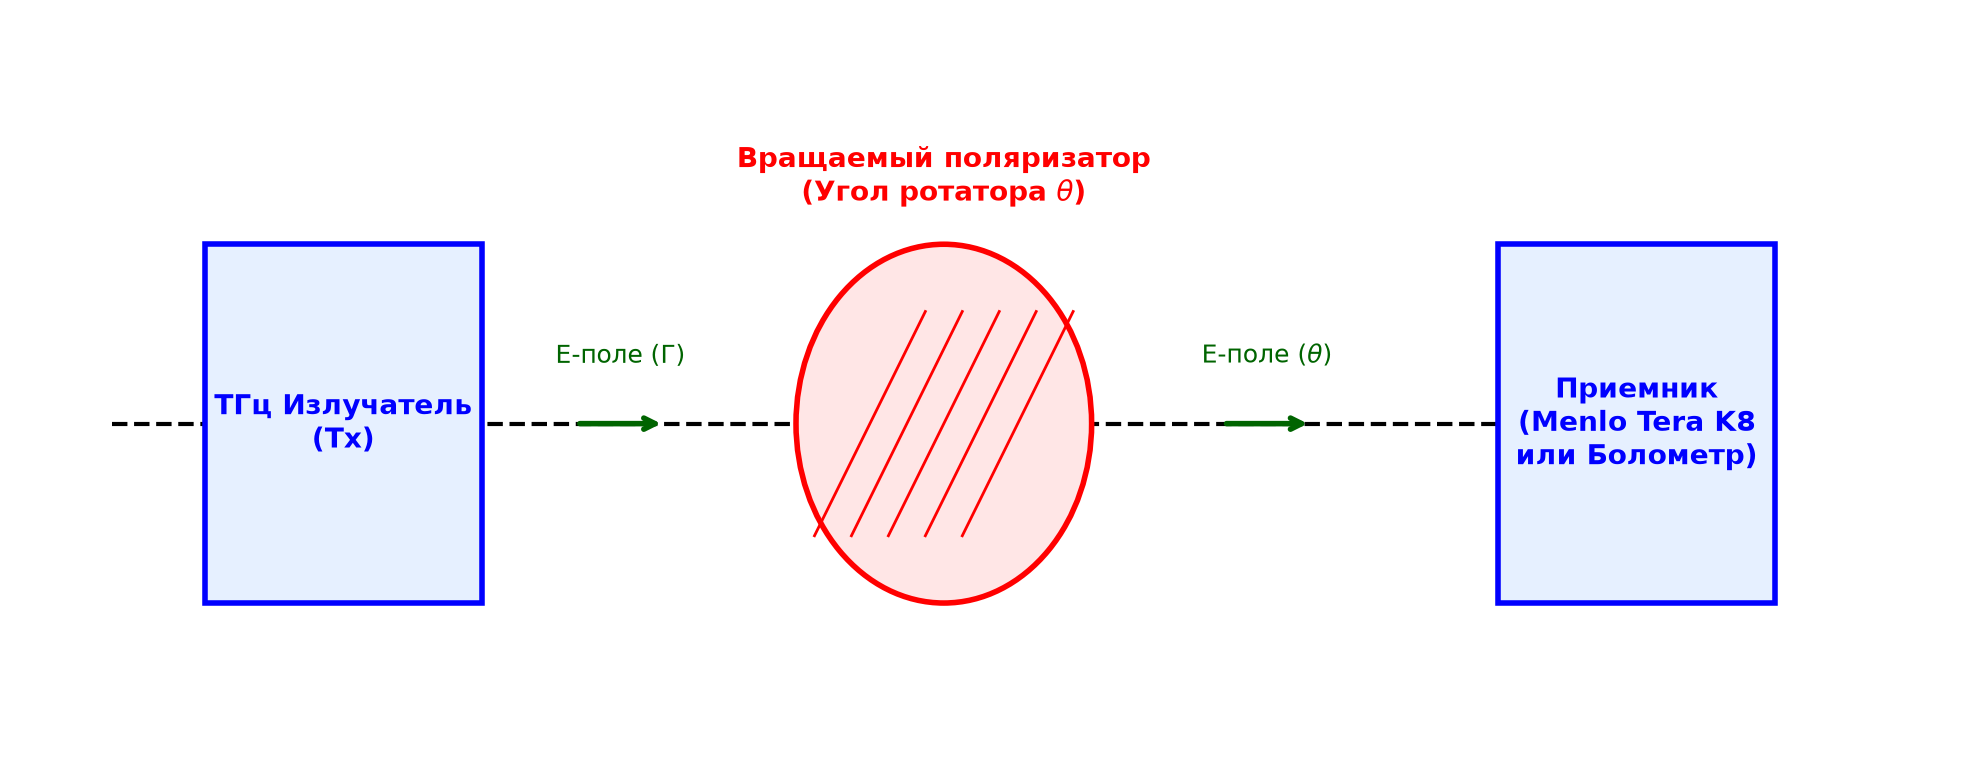
\includegraphics[width=0.62\textwidth]{fig0_1}
		\vspace{-0.5em}
		\caption{Схема экспериментальной установки для калибровки аттенюатора.}
		\label{fig:scheme}
	\end{figure}
	
	\vspace{-0.5em}
	
	\noindent\textbf{4. Сценарии применения аттенюатора} \\
	В зависимости от типа детектора и оптического тракта вносимое ослабление рассчитывается по одному из двух сценариев:
	\begin{enumerate}[leftmargin=0.8cm, label=\Alph*., itemsep=2pt]
		\item \textbf{Сценарий А (Болометр / Ячейка Голея) --- нечувствительный к поляризации приемник}: \\
		Измеряется полная прошедшая мощность. Затухание подчиняется закону Малюса ($\cos^2$ по мощности):
		$$T(\theta) = T_{\text{open}} \cos^2(\theta - \theta_{\text{offset}}) + T_{\text{noise}}$$
		Азимут плоскости поляризации на выходе равен углу установки ротатора $\theta$.
		
		\item \textbf{Сценарий Б (ФПА Menlo Tera K8) --- чувствительный к поляризации приемник}: \\
		Приемная антенна чувствительна только к горизонтальному полю. Двойное проецирование поля на сетки возводит закон Малюса по мощности в квадрат ($\cos^4$ по мощности):
		$$T(\theta) = T_{\text{open}} \cos^4(\theta - \theta_{\text{offset}}) + T_{\text{noise}}$$
		Азимут выходной поляризации зафиксирован горизонтально (по оси приемника). При этом вносится дополнительное затухание за счет фильтрации ортогональной компоненты.
	\end{enumerate}
	
	\newpage
	
	% ==========================================
	% СТРАНИЦА 2: КАЛИБРОВОЧНЫЕ ГРАФИКИ И ПОГРЕШНОСТИ
	% ==========================================
	\begin{center}
		{\color{headerblue}\large\bfseries КАЛИБРОВОЧНЫЕ КАРТЫ И ПОГРЕШНОСТИ АТТЕНЮАТОРА}
	\end{center}
	
	\vspace{0.3em}
	
	\noindent\textbf{5.  Калибровочные кривые пропускания и ослабления} \\
	Для быстрой ручной настройки затухания используйте графические кривые для частот 0.5 ТГц и 1.0 ТГц. Шкала частот по верхней границе продублирована в длинах волн ($\lambda = c / \nu$).
	
	\begin{figure}[H]
		\centering
		
\includegraphics[width=0.85\textwidth]{passport_calibration}
		\vspace{-0.5em}
		\caption{Калибровочные кривые: малые затухания в линейной шкале (слева) и глубокие затухания в децибельной шкале (справа). Правые шкалы показывают альтернативные единицы измерения.}
		\label{fig:calib}
	\end{figure}
	
	\vspace{-0.8em}
	
	\noindent\textbf{6. Анализ погрешности и углового люфта} \\
	Погрешность вносимого затухания $\Delta A$ (в дБ) складывается из систематической погрешности модели ($\approx 1.4$~дБ) и погрешности установки угла ротатора $\Delta \theta$ (люфт лимба). Из-за тригонометрического характера закона Малюса чувствительность затухания к угловым ошибкам резко возрастает при глубоких ослаблениях ($\theta > 70^\circ$).
	
	\begin{figure}[H]
		\centering
		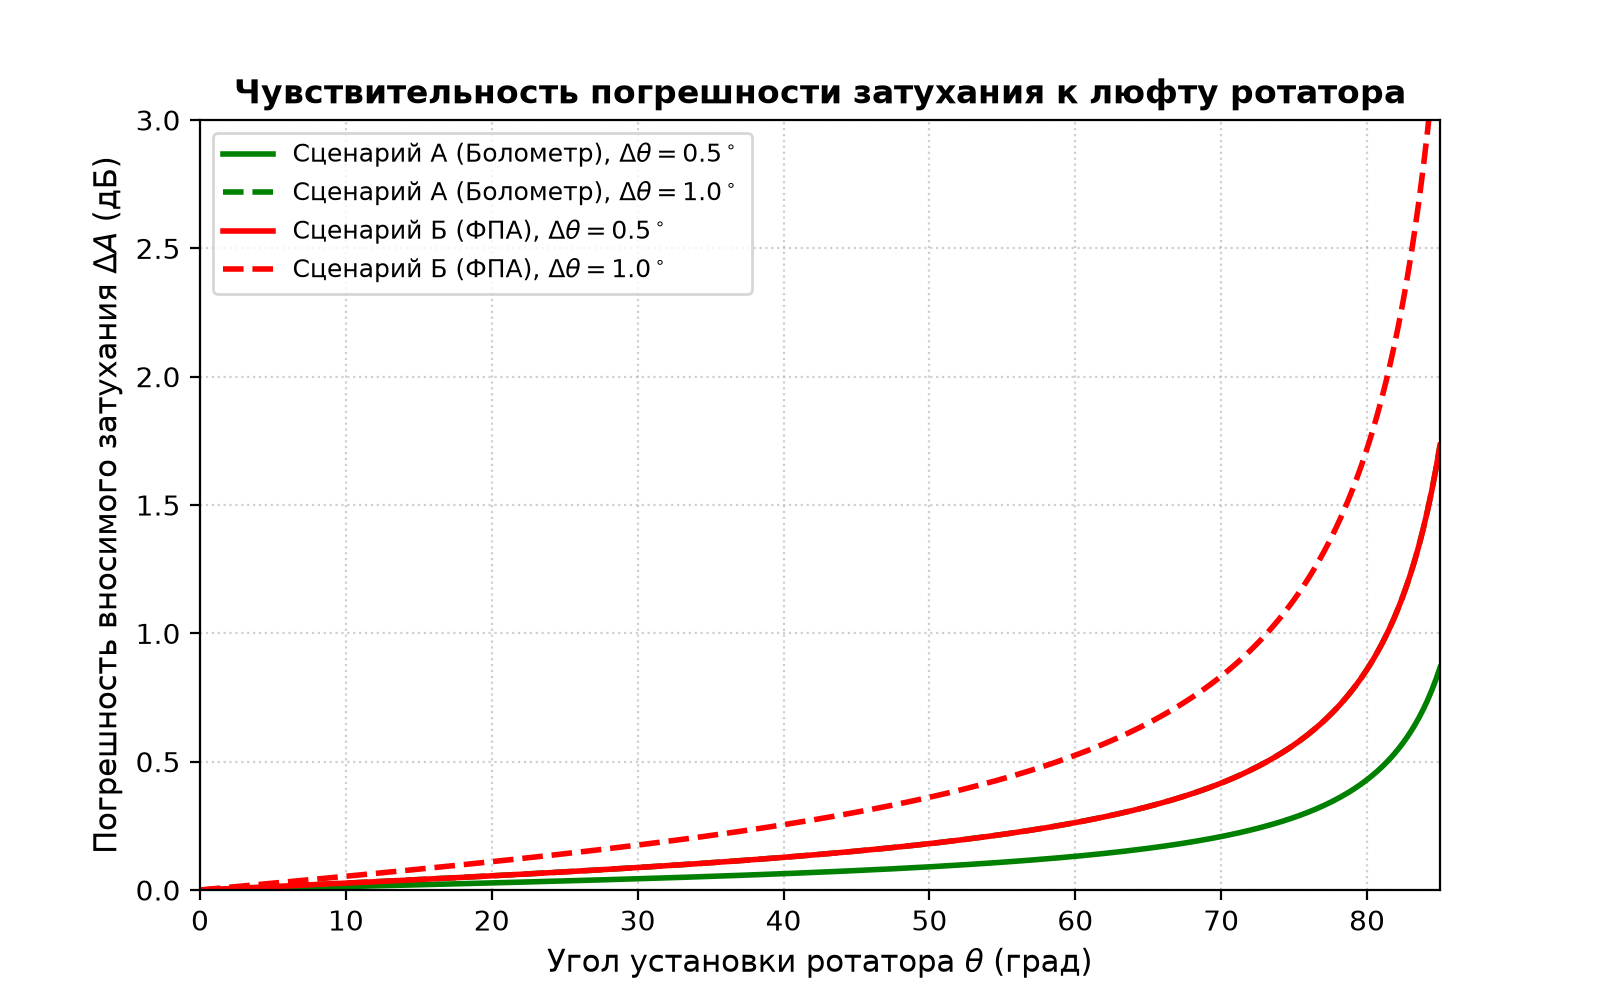
\includegraphics[width=0.45\textwidth]{passport_error}
		\vspace{-0.5em}
		\caption{Зависимость погрешности ослабления $\Delta A$ от угла установки при люфте лимба ротатора $\Delta\theta = 0.5^\circ$ и $1.0^\circ$.}
		\label{fig:error}
	\end{figure}
	
	\vspace{-0.8em}
	
	\noindent\textbf{7. Физические ограничения и СВЧ-диапазон}
	\begin{itemize}[leftmargin=0.6cm, itemsep=2pt]
		\item \textbf{Дифракция на оправе}: Решетка сохраняет поляризационные свойства на любых низких частотах. Однако на частотах ниже 10 ГГц ($\lambda > 3$ см) длина волны становится сопоставимой с диаметром световой апертуры оправы ($85$ мм), что приводит к краевой дифракции пучка и нарушению плоского фронта.
		\item \textbf{Спектральный шумовой пол}: Глубина ослабления на углах вблизи $90^\circ$ ограничена шумовым порогом вашей ТГц-установки (для Menlo Tera K8 составляет около $-36$ дБ на 1.0 ТГц и $-46$ дБ на 0.3 ТГц).
	\end{itemize}
	
	\vspace{0.3em}
	\hrule
	\vspace{0.3em}
	\begin{center}
		\footnotesize
		Свидетельство выдано на основании исследований в рамках проекта \textit{«THz-Spectroscopy-Python-Manual2»}. \\
		Калибровка произведена: 29 июня 2026~г. \quad | \quad Действительно до: 29 июня 2028~г. \\
		\vspace{0.3em}
		\textbf{Лаборатория терагерцовой спектроскопии} \hfill \textbf{Подпись поверителя: \underline{\hspace{4cm}}}
	\end{center}
	
\end{document}
